%==============================================================================
%  Supplementary File S1 — Supplementary methods
%  Companion to main_applsci.tex. Compiles standalone; export to DOCX for submission.
%  Contains Figure S1 (detailed pipeline architecture), referenced from
%  Methods > Statistical Criteria to SQL Transformation Pipeline.
%  Requires pgf/pgfplots as configured for main_rt.tex.
%==============================================================================
\documentclass[10pt]{article}
\usepackage[utf8]{inputenc}
\usepackage[T1]{fontenc}
\usepackage[margin=0.9in]{geometry}
\usepackage{times}
\usepackage{booktabs}
\usepackage{array}
\usepackage{amsmath}
\usepackage{xcolor}
\usepackage{caption}
\usepackage{enumitem}
\usepackage{tikz}
\usetikzlibrary{shapes.geometric,arrows.meta,positioning,fit,backgrounds,calc}
\usepackage[colorlinks=true,allcolors=blue!55!black]{hyperref}

\newcommand{\PH}[1]{{\color{red}\textbf{[#1]}}}
\newcolumntype{L}[1]{>{\raggedright\arraybackslash}p{#1}}
\newcolumntype{C}[1]{>{\centering\arraybackslash}p{#1}}
\captionsetup{labelsep=period,font=small,justification=justified,
              singlelinecheck=false,skip=4pt}
\setcounter{secnumdepth}{0}
\pagestyle{plain}
\renewcommand{\thefigure}{S\arabic{figure}}
\renewcommand{\thetable}{S\arabic{table}}

\begin{document}

\begin{center}
{\large\bfseries Supplementary File S1. Supplementary methods}\\[2pt]
{\footnotesize Companion to: \emph{Metadata-Grounded Large Language Models for Converting Hospital Statistical
Requests into Clinical Data Warehouse Queries}}
\end{center}

%==============================================================================
\section{S1. Detailed pipeline architecture}
%==============================================================================

\begin{figure}[h]
\caption{Detailed architecture of the automated transformation pipeline. Solid
arrows carry structured JSON between modules; dashed arrows are retrieval or
lookup calls into the metadata knowledge base; the dotted arrow is the
verification feedback path. CDW: clinical data warehouse; DC: data center; DL:
data lake; KB: knowledge base; LLM: large language model; MDR: master data
repository; NL: natural language.}
\label{fig:s1}
\centering
\vspace{2pt}

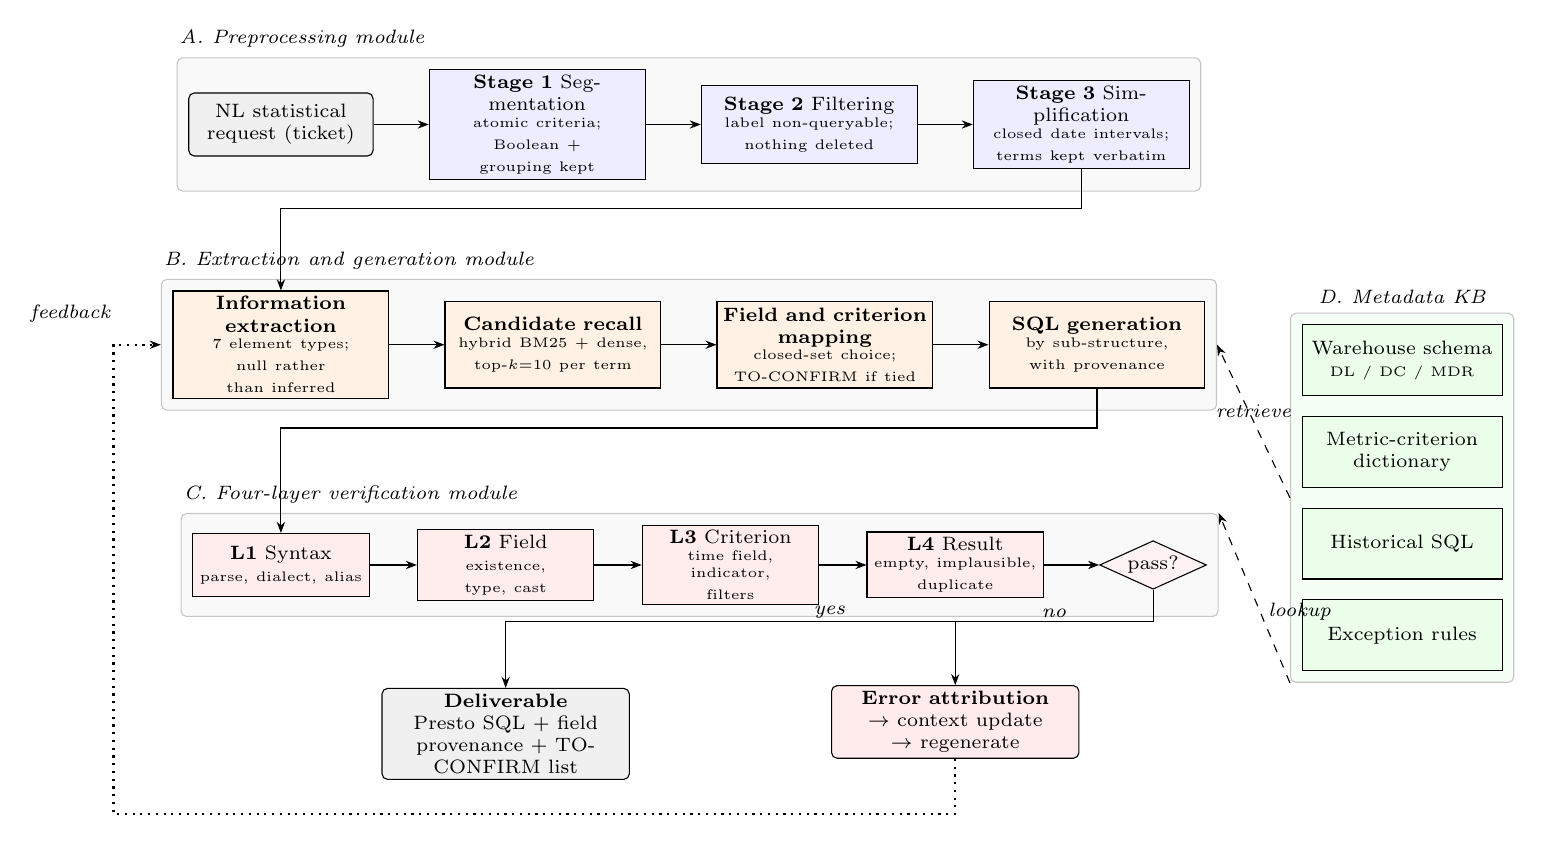
\begin{tikzpicture}[
  font=\scriptsize,
  node distance=4mm and 7mm,
  lane/.style ={draw=gray!45,fill=gray!5,rounded corners=2pt,inner sep=4pt},
  io/.style   ={draw,rounded corners=2pt,fill=gray!12,align=center,
                text width=22mm,minimum height=8mm,inner sep=2pt},
  st/.style   ={draw,fill=blue!7,align=center,text width=26mm,
                minimum height=10mm,inner sep=2pt},
  mod/.style  ={draw,fill=orange!10,align=center,text width=26mm,
                minimum height=11mm,inner sep=2pt},
  kb/.style   ={draw,fill=green!8,align=center,text width=24mm,
                minimum height=9mm,inner sep=2pt},
  chk/.style  ={draw,fill=red!7,align=center,text width=21mm,
                minimum height=8mm,inner sep=2pt},
  dec/.style  ={draw,diamond,aspect=2.2,align=center,inner sep=1pt,fill=red!5},
  lbl/.style  ={font=\scriptsize\itshape,inner sep=1pt},
  >={Stealth[length=4pt]}]

%---------------- Lane A : preprocessing ----------------
\node[io] (req) {NL statistical\\request (ticket)};
\node[st, right=of req] (s1) {\textbf{Stage 1} Segmentation\\{\tiny atomic criteria;\\Boolean + grouping kept}};
\node[st, right=of s1]  (s2) {\textbf{Stage 2} Filtering\\{\tiny label non-queryable;\\nothing deleted}};
\node[st, right=of s2]  (s3) {\textbf{Stage 3} Simplification\\{\tiny closed date intervals;\\terms kept verbatim}};
\draw[->] (req)--(s1); \draw[->] (s1)--(s2); \draw[->] (s2)--(s3);
\begin{scope}[on background layer]
\node[lane,fit=(req)(s1)(s2)(s3)] (laneA) {};
\end{scope}
\node[lbl,anchor=south west,yshift=0.8mm] at (laneA.north west) {A. Preprocessing module};

%---------------- Lane B : extraction and mapping ----------------
\node[mod, below=17mm of req.south, anchor=north] (ie)
  {\textbf{Information extraction}\\{\tiny 7 element types;\\null rather than inferred}};
\node[mod, right=of ie] (rec)
  {\textbf{Candidate recall}\\{\tiny hybrid BM25 + dense,\\top-$k$=10 per term}};
\node[mod, right=of rec] (map)
  {\textbf{Field and criterion}\\\textbf{mapping}\\{\tiny closed-set choice;\\TO-CONFIRM if tied}};
\node[mod, right=of map] (gen)
  {\textbf{SQL generation}\\{\tiny by sub-structure,\\with provenance}};
\draw[->] (s3.south) -- ++(0,-5mm) -| (ie.north);
\draw[->] (ie)--(rec); \draw[->] (rec)--(map); \draw[->] (map)--(gen);
\begin{scope}[on background layer]
\node[lane,fit=(ie)(rec)(map)(gen)] (laneB) {};
\end{scope}
\node[lbl,anchor=south west,yshift=0.8mm] at (laneB.north west) {B. Extraction and generation module};

%---------------- Lane C : verification ----------------
\node[chk, below=17mm of ie.south, anchor=north] (v1) {\textbf{L1} Syntax\\{\tiny parse, dialect, alias}};
\node[chk, right=6mm of v1] (v2) {\textbf{L2} Field\\{\tiny existence, type, cast}};
\node[chk, right=6mm of v2] (v3) {\textbf{L3} Criterion\\{\tiny time field, indicator,\\filters}};
\node[chk, right=6mm of v3] (v4) {\textbf{L4} Result\\{\tiny empty, implausible,\\duplicate}};
\node[dec, right=7mm of v4] (pass) {pass?};
\draw[->] (gen.south) -- ++(0,-5mm) -| (v1.north);
\draw[->] (v1)--(v2); \draw[->] (v2)--(v3); \draw[->] (v3)--(v4); \draw[->] (v4)--(pass);
\begin{scope}[on background layer]
\node[lane,fit=(v1)(v2)(v3)(v4)(pass)] (laneC) {};
\end{scope}
\node[lbl,anchor=south west,yshift=0.8mm] at (laneC.north west) {C. Four-layer verification module};

%---------------- Outputs ----------------
\node[io, below=11mm of v2.south, anchor=north, text width=30mm] (out)
  {\textbf{Deliverable}\\Presto SQL + field provenance + TO-CONFIRM list};
\node[io, below=11mm of v4.south, anchor=north, text width=30mm, fill=red!8] (err)
  {\textbf{Error attribution}\\$\to$ context update $\to$ regenerate};
\draw[->] (pass.south) -- ++(0,-4mm) -| node[lbl,pos=0.25,above]{yes} (out.north);
\draw[->] (pass.south) -- ++(0,-4mm) -| node[lbl,pos=0.25,above]{no}  (err.north);
% feedback path: routed down and around the left margin so it crosses no box
\coordinate (fbA) at ($(err.south)+(0,-7mm)$);
\coordinate (fbB) at ($(laneB.west)+(-6mm,0)$);
\draw[->,dotted,thick] (err.south) -- (fbA) -| (fbB) -- (laneB.west);
\node[lbl,anchor=east] at ($(fbB)+(0,4mm)$) {feedback};

%---------------- Knowledge base (right column) ----------------
\node[kb, right=12mm of pass, yshift=26mm] (kb1) {Warehouse schema\\{\tiny DL / DC / MDR}};
\node[kb, below=2.5mm of kb1] (kb2) {Metric-criterion\\dictionary};
\node[kb, below=2.5mm of kb2] (kb3) {Historical SQL};
\node[kb, below=2.5mm of kb3] (kb4) {Exception rules};
\begin{scope}[on background layer]
\node[lane,fill=green!4,fit=(kb1)(kb2)(kb3)(kb4)] (laneD) {};
\end{scope}
\node[lbl,anchor=south,yshift=0.8mm] at (laneD.north) {D. Metadata KB};

% KB access: lane-to-lane connectors on the right, crossing no box
\draw[->,dashed] (laneD.west) -- node[lbl,above,pos=0.5]{retrieve} (laneB.east);
\draw[->,dashed] (laneD.south west) -- node[lbl,above right,pos=0.35]{lookup} (laneC.north east);

\end{tikzpicture}
\end{figure}

%==============================================================================
\section{S2. Processing procedures in detail}
%==============================================================================

\subsection{S2.1 Preprocessing}
Segmentation splits the request on sentence and list boundaries and on
enumerated markers, then re-attaches trailing qualifiers to the criterion they
modify. Boolean connectives and grouping hierarchy are recorded as structure
rather than resolved, so that a later stage cannot silently change precedence.
Filtering labels rather than deletes, so that the count of dropped elements is
auditable; a criterion is non-queryable when it expresses formatting, delivery,
justification, or preference rather than a data condition. Simplification
rewrites each surviving criterion into one sentence and normalizes every
temporal expression to a closed interval $[\,t_{0},t_{1})$ resolved against the
report date; clinical and administrative terms are never replaced by synonyms at
this stage, because synonym substitution is the dominant source of downstream
criterion drift.

\subsection{S2.2 Candidate recall}
For each business term, candidates are scored as
\[
\text{Score}(c)=\alpha\,\text{Score}_{\text{key}}(c,Q)
+\beta\,\text{Score}_{\text{sem}}(c,Q)
+\gamma\,\text{Score}_{\text{hist}}(c,Q),
\]
combining BM25 keyword match over column names and annotations, dense
sentence-embedding similarity, and a historical-SQL hit term that rewards
tables, columns, and join paths appearing in engineer-certified queries for the
same indicator family. The top $k=8$ candidates are passed to the mapping step.
Weights used in all reported experiments: $\alpha=0.30$ (keyword), $\beta=0.30$ (semantic), $\gamma=0.40$ (historical SQL); the historical-SQL term
carries the largest weight because a validated join path is stronger evidence
than lexical or embedding similarity.

\subsection{S2.3 Mapping and the TO-CONFIRM rule}
Mapping is a closed-set choice over the recalled candidates. The model may not
emit an identifier that is absent from the candidate set. When two or more
candidate counting criteria are defensible for the same indicator, the model is
required to abstain and emit a TO-CONFIRM item naming the competing candidates
and the distinguishing property. Abstention is scored as a success in the
criterion dimension and as a non-delivery in the throughput dimension, so the
system is not rewarded for abstaining indiscriminately.

\subsection{S2.4 Four-layer verification}
Layer 1 parses the statement and checks dialect and alias validity. Layer 2
checks that every table and column exists, that qualification is correct, and
that every comparison against a VARCHAR column carries an explicit cast. Layer 3
checks the counting criterion against the metric-criterion dictionary, including
the time field, the inclusion and exclusion sets, and the grouping granularity.
Layer 4 executes the statement and inspects the result for emptiness,
implausible magnitude relative to the historical series for the same indicator,
and unexpected duplication. On failure the error is attributed to a module, the
retrieval context is updated, and generation is repeated.

%==============================================================================
\section{S3. Task set composition}
%==============================================================================

\begin{table}[h]\centering
\caption{Composition of the three task sets.}
\footnotesize
\begin{tabular}{@{}L{4.6cm}C{2.2cm}C{2.2cm}C{2.2cm}@{}}
\toprule
& Development & Validation & Main study\\
\midrule
Tasks, n                         & 30  & 7   & 24\\
Purpose                          & dictionary and prompt construction & end-to-end system evaluation & factorial model $\times$ prompt comparison\\
Surgery and anesthesia, n        & 10  & 3   & 7\\
Blood transfusion, n             & 10  & 1   & 5\\
Laboratory, n                    & 10  & 1   & 5\\
Medical record and case mix, n   & 0   & 1   & 4\\
Other, n                         & 0   & 1   & 3\\
\addlinespace
Simple, n                        & 12 & 2 & 10\\
Moderate, n                      & 11 & 3 & 9\\
Complex, n                       & 7  & 2 & 5\\
\addlinespace
Business terms extracted, n & 398 & 158 & 276\\
Executed against                 & --- & production CDW & SynHDW\\
\bottomrule
\end{tabular}
\end{table}

\noindent
Complexity strata are defined by join depth and criterion sensitivity: simple =
one table and at most one filter; moderate = two tables with multiple filters;
complex = three or more tables, or any indicator whose counting criterion has
more than one defensible reading. The development and evaluation sets are
disjoint at the task level and at the indicator level; no development exemplar
was reused as an evaluation item.

%==============================================================================
\section{S4. SynHDW construction}
%==============================================================================
SynHDW is a de-identified synthetic mirror of the warehouse. Table and column
names, types, and logical-deletion and organization-code conventions are copied
from production; row content is generated. Coverage is deliberately partial
($\sim$1680 of the $>$13{,}000 production columns), which is what makes it a test
bed for hallucination: a model that invents an identifier, or that reaches for a
column it remembers from pretraining rather than one that is present, fails
detectably. Population rates for flag columns were sampled to reproduce the
production profile, including the flag columns that are unpopulated in
production, so that the unpopulated-flag failure mode is reproducible.
Generation seed: 20251118. Row counts: 112{,}680 synthetic patients, 742{,}000 visits, 368{,}000 surgical records, 86{,}400 transfusion records, 10{,}850{,}000 laboratory results, covering 2019--2023.

%==============================================================================
\section{S5. Hallucination detection algorithm}
%==============================================================================
\begin{enumerate}[leftmargin=1.6em,itemsep=1pt,topsep=2pt]
  \item Parse the generated statement and collect every table reference, column
        reference, and literal in an identifier position.
  \item Resolve each reference against the SynHDW metadata inventory. An
        unresolvable reference is \textbf{Category A}.
  \item For each resolved column, compare its owning table and subject domain
        with the resolved mapping entry. A mismatch in the counting criterion
        --- the time field, the indicator definition, or the filter set --- is
        \textbf{Category B}.
  \item Detect natural-language tokens in identifier positions by checking for
        characters outside the identifier character class or for tokens present
        in the business-term lexicon but absent from the column lexicon. These
        are \textbf{Category C}.
  \item Detect placeholder literals by pattern (angle brackets, ellipses,
        \verb|your_|, \verb|TODO|, \verb|xxx|, and the model-specific patterns
        listed in the detector configuration shipped with the code). These are
        \textbf{Category D}.
  \item Remaining defects that a mechanical rewrite can repair --- missing
        logical-deletion filter, missing organization-code filter, wrong
        function name, absent cast --- are \textbf{Category E}.
  \item A query is counted as hallucinating if it contains at least one defect
        of any category. The hallucination rate is the proportion of
        \emph{generated} queries so counted; the effective SQL rate is
        $\text{generation rate}\times(1-\text{hallucination rate})$.
\end{enumerate}

\noindent
\textbf{Counting convention.} A hallucinating query is assigned exactly one
category --- the most severe defect it contains, under the severity order
A $>$ B $>$ C $>$ D $>$ E. One query therefore contributes one unit to exactly one
cell of Table 5 in the main text. Consequently the per-model row totals in
Table 5 equal the number of hallucinating queries for that model, the grand
total equals the number of hallucinating queries overall, and the reported
overall hallucination rate is that grand total divided by the number of
generated queries. Figure 4 in the main text plots the same counts.

\vspace{4pt}
\noindent
Detection was validated against manual adjudication on a random sample of 72 queries; agreement between the automated classifier and the adjudicators was 0.88.

\vspace{6pt}
\noindent
\textbf{Auditable basis.} Every rate reported in Table 4 and Figure 3 of the main
text derives from the two integer counts in Table~\ref{tab:basis}: each model
received 24 tasks $\times$ 5 prompting strategies = 120 attempts. SQL generation
rate is $\text{generated}/120$; hallucination rate is
$\text{hallucinating}/\text{generated}$; effective SQL rate is the product of the
first with $(1-\text{second})$. No reported percentage is independent of these
counts, so the whole numeric spine can be recomputed from this table alone.

\begin{table}[h]\centering
\caption{Integer basis for all model-level rates.}
\label{tab:basis}
\footnotesize
\begin{tabular}{@{}L{3.4cm}L{1.9cm}L{2.2cm}L{2.0cm}L{2.0cm}L{2.0cm}@{}}
\toprule
Model & Attempts, n & Generated, n & Hallucinating, n & Generation, \% & Effective, \%\\
\midrule
qwen2.5:7b        & 120 & 108 & 22 & 90.0 & 71.7\\
deepseek-v3       & 120 & 115 & 35 & 95.8 & 66.7\\
glm4:9b           & 120 & 118 & 40 & 98.3 & 65.0\\
gpt-4o            & 120 & 117 & 44 & 97.5 & 60.8\\
deepseek-r1:7b    & 120 & 102 & 34 & 85.0 & 56.7\\
llama3:8b         & 120 & 105 & 48 & 87.5 & 47.5\\
claude-3.5-sonnet & 120 & 104 & 49 & 86.7 & 45.8\\
phi3              & 120 & 22  & 2  & 18.3 & 16.7\\
\midrule
Total             & 960 & 791 & 274 & 82.4 & ---\\
\bottomrule
\end{tabular}
\end{table}

\noindent
The overall hallucination rate reported in the main text is
$274/791=34.6\%$, and the one-way ANOVA over model-level effective rates carries $df=(7,783)$. Phi3's hallucination rate is computed on only 22 generated queries
and is therefore reported with an explicit caveat rather than read as a strength.

\end{document}
